%%%%%%%%%%%%%%%%%%%%%%%%%%%%%%%%%%%%%%%%%%%%%%%%%%%%%%%%%%%%%%%%%%%%
% Overivew
%%%%%%%%%%%%%%%%%%%%%%%%%%%%%%%%%%%%%%%%%%%%%%%%%%%%%%%%%%%%%%%%%%%%

\section{Model Interlocking Assemblies}
\label{sec:model}



In this section, we introduce our conceptual representation of interlocking assemblies using a family of directed graphs. We show how this graph-based representation leads to an efficient algorithm to {\em test} interlocking. 
In Section~\ref{sec:approach} we then explain how to effectively employ this representation and algorithm to {\em design} interlocking assemblies.
%\TODO{one more assumption: we focus on (dis)assemblies parts with translational motions, e.g., do not consider taking a part by rotating it first and then doing the translation.}


\begin{figure}[!t]
	\centering
	%\vspace*{-3.5mm}
	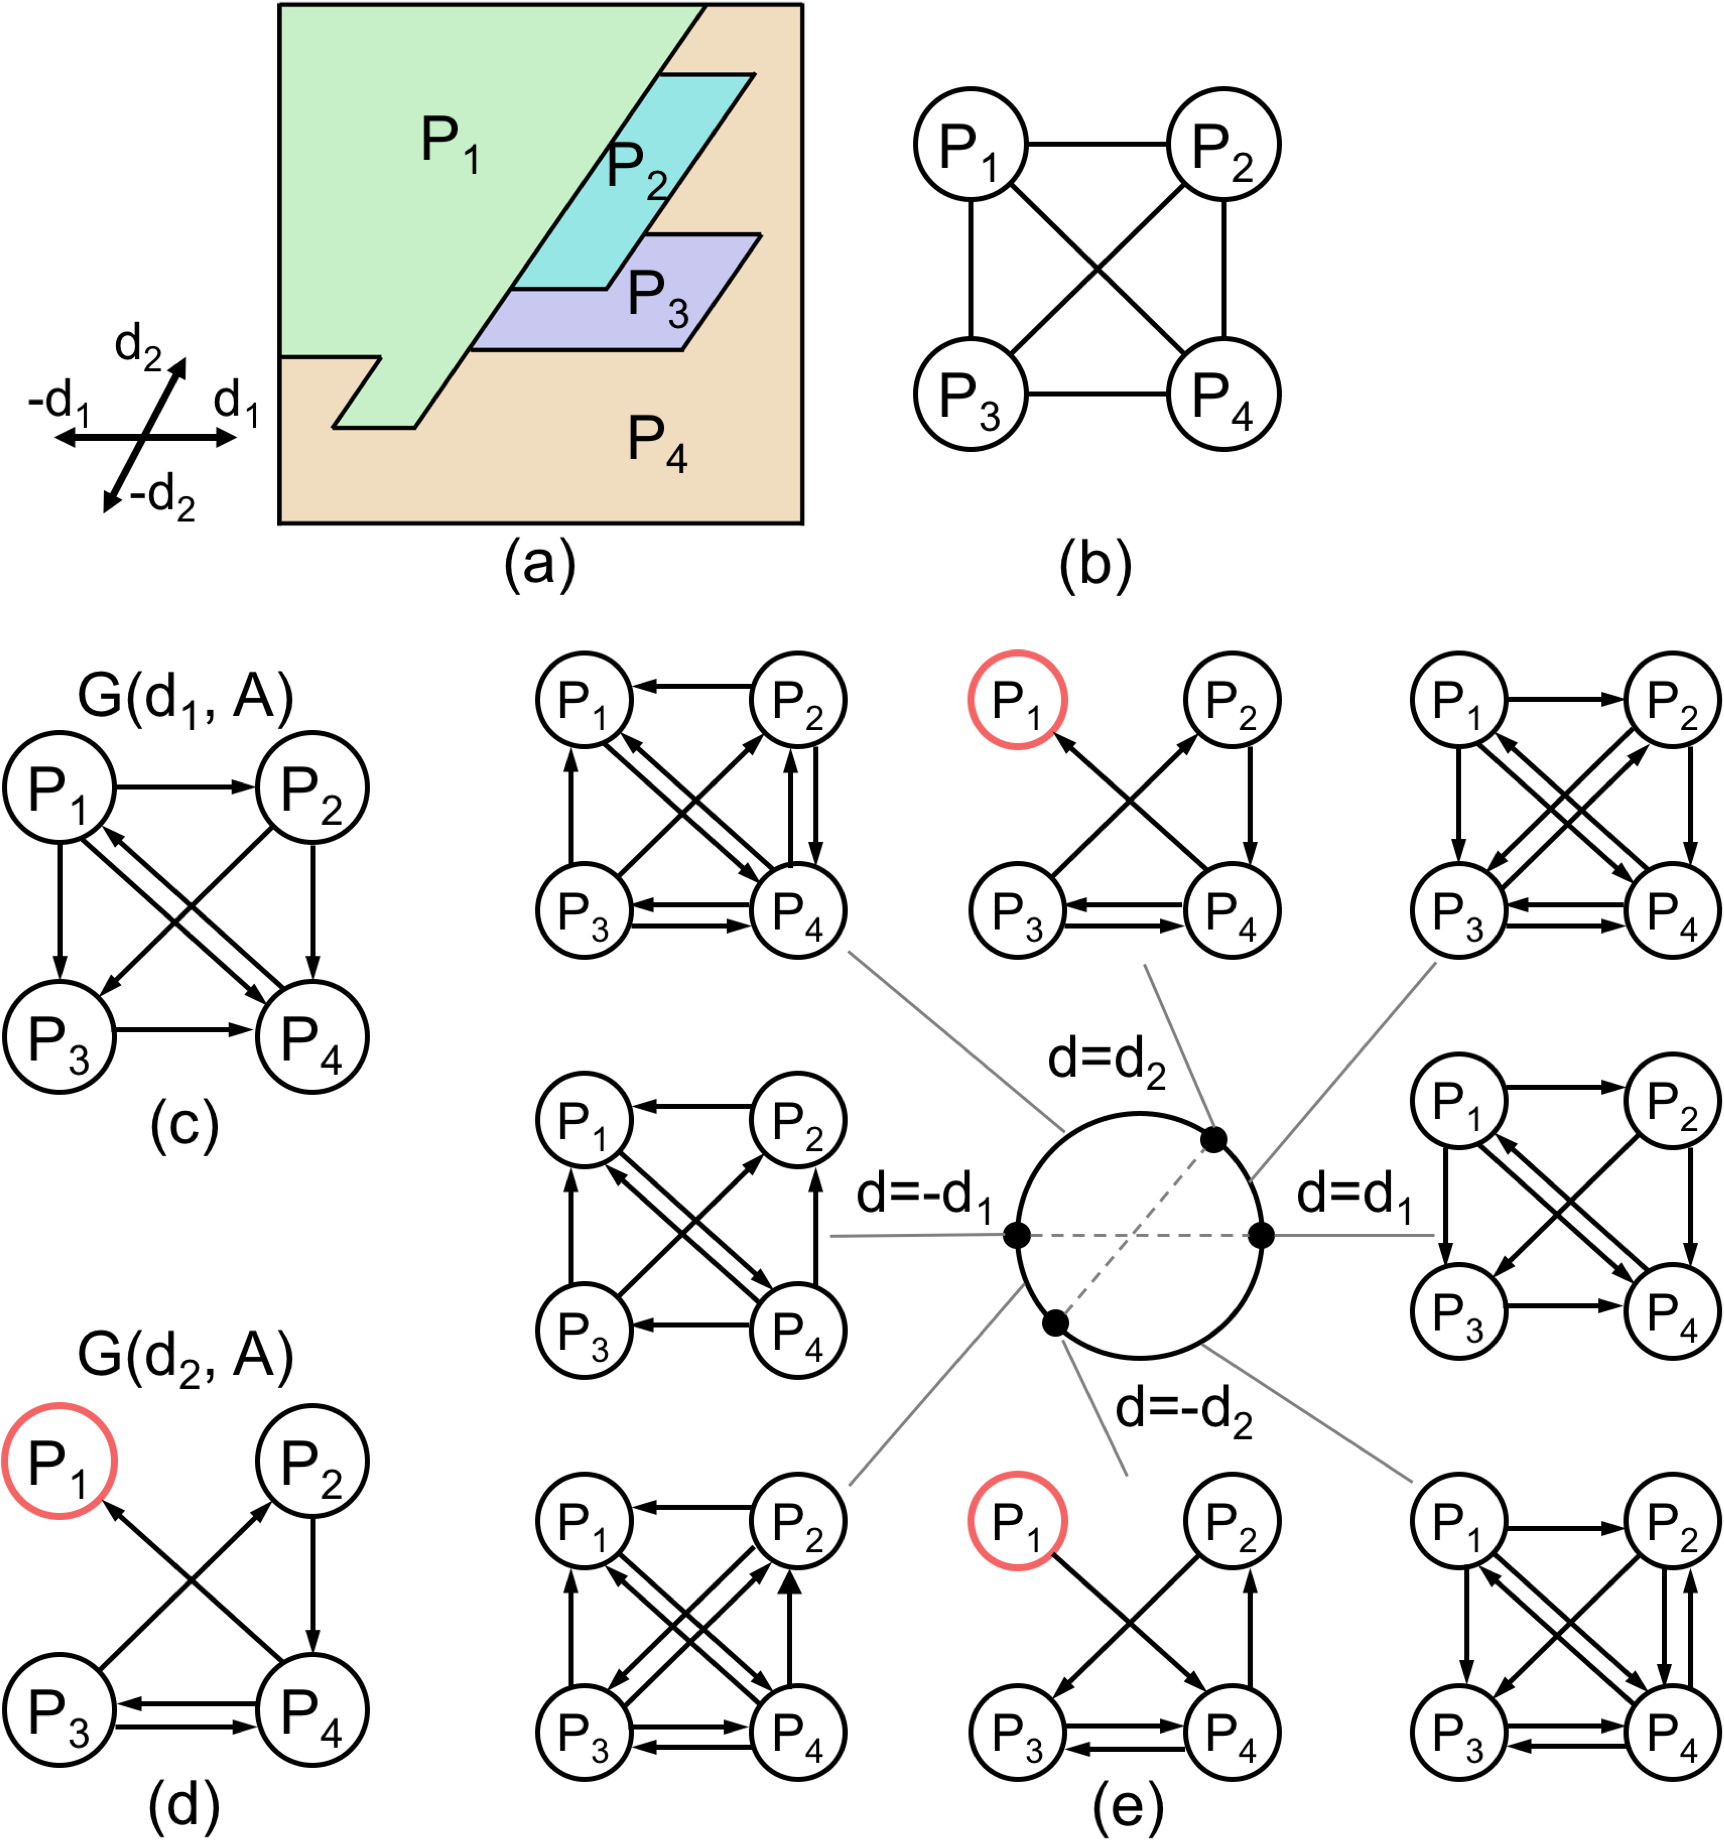
\includegraphics[width=8.00cm]{images/NDBG.png}
	\vspace*{-2.5mm}
	\caption{Example DBGs and NDBG.
		(a\&b) A 2D interlocking assembly and its parts-graph, where the key $P_1$ is movable along $d_2$;
		(c\&d) Two DBGs of the assembly; and
		(e) NDBG of the assembly.
		A part with zero out-degree or in-degree in a DBG is highlighted with a red circle. 
		%\Mark{I would still consider using crossing edges, I think it will make it easier to read.I would also expand the figure  to reach to full width, i.e. add more space.}
	}
	\vspace*{-4.0mm}
	\label{fig:NDBG}
\end{figure}



\subsection{Graph Model}

%%%%%%%%%%%%%%%%%%%%%%%%%%%%%%%%%%%%%%%%%%%%%%%%
% Our Inputs
%%%%%%%%%%%%%%%%%%%%%%%%%%%%%%%%%%%%%%%%%%%%%%%%

Consider an assembly $\mathbf{A}$, made of $n$ parts $P_1$, $...$, $P_n$.
We make the following assumptions:
1) each part $P_i$ is rigid; 
2) neighboring parts have planar surface contact only; and 
%(e.g., corner-surface and edge-surface contacts are not considered); and
3) $\mathbf{A}$ can be disassembled by single-part translational motions, i.e., part rotation is not required and all other parts remain fixed when removing a part.


%%%%%%%%%%%%%%%%%%%%%%%%%%%%%%%%%%%%%%%%%%%%%%%%
% Base DBGs
%%%%%%%%%%%%%%%%%%%%%%%%%%%%%%%%%%%%%%%%%%%%%%%%

\vspace*{1.0mm}
\noindent
{\bf Directional Blocking Graph (DBG).}\  
We denote as $G(d, A)$ the {\em directional blocking graph} of assembly $\mathbf{A}$ for translation along direction $d$. 
This directed graph has nodes representing the parts of $\mathbf{A}$ and directed edges $e_{i \rightarrow j}$ from $P_i$ to $P_j$  if and only if $P_j$ prevents any translational motion of $P_i$ along $d$. 
In other words, $e_{i \rightarrow j}$ can be read as ``$P_i$  is blocked by $P_j$" in direction $d$. 
See Figure~\ref{fig:NDBG}(c\&d) for two examples.

If $G(d, A)$ is {\em strongly connected}, i.e. if every node can be reached from every other node, no part or part group is movable along $d$; see Figure~\ref{fig:NDBG}(c). 
A part group $\mathbf{S}$ of $\mathbf{A}$ is locally free to translate in direction $d$ ($-d$), if and only if the out-degree (in-degree) of $\mathbf{S}$ in $G(d, A)$ is zero; see $P_1$ in Figure~\ref{fig:NDBG}(d).
%there is no edge in $G(d, A)$ connecting parts in $\mathbf{S}$ to parts in $\mathbf{A} \setminus \mathbf{S}$; see $P_1$ in Figure~\ref{fig:NDBG}(d) for an example.
%since there is no out-edge connecting it with the other nodes in the graph; see Figure~\ref{fig:NDBG}(d). 

\begin{figure*}[!t]
	\centering
	%\vspace*{-3.5mm}
	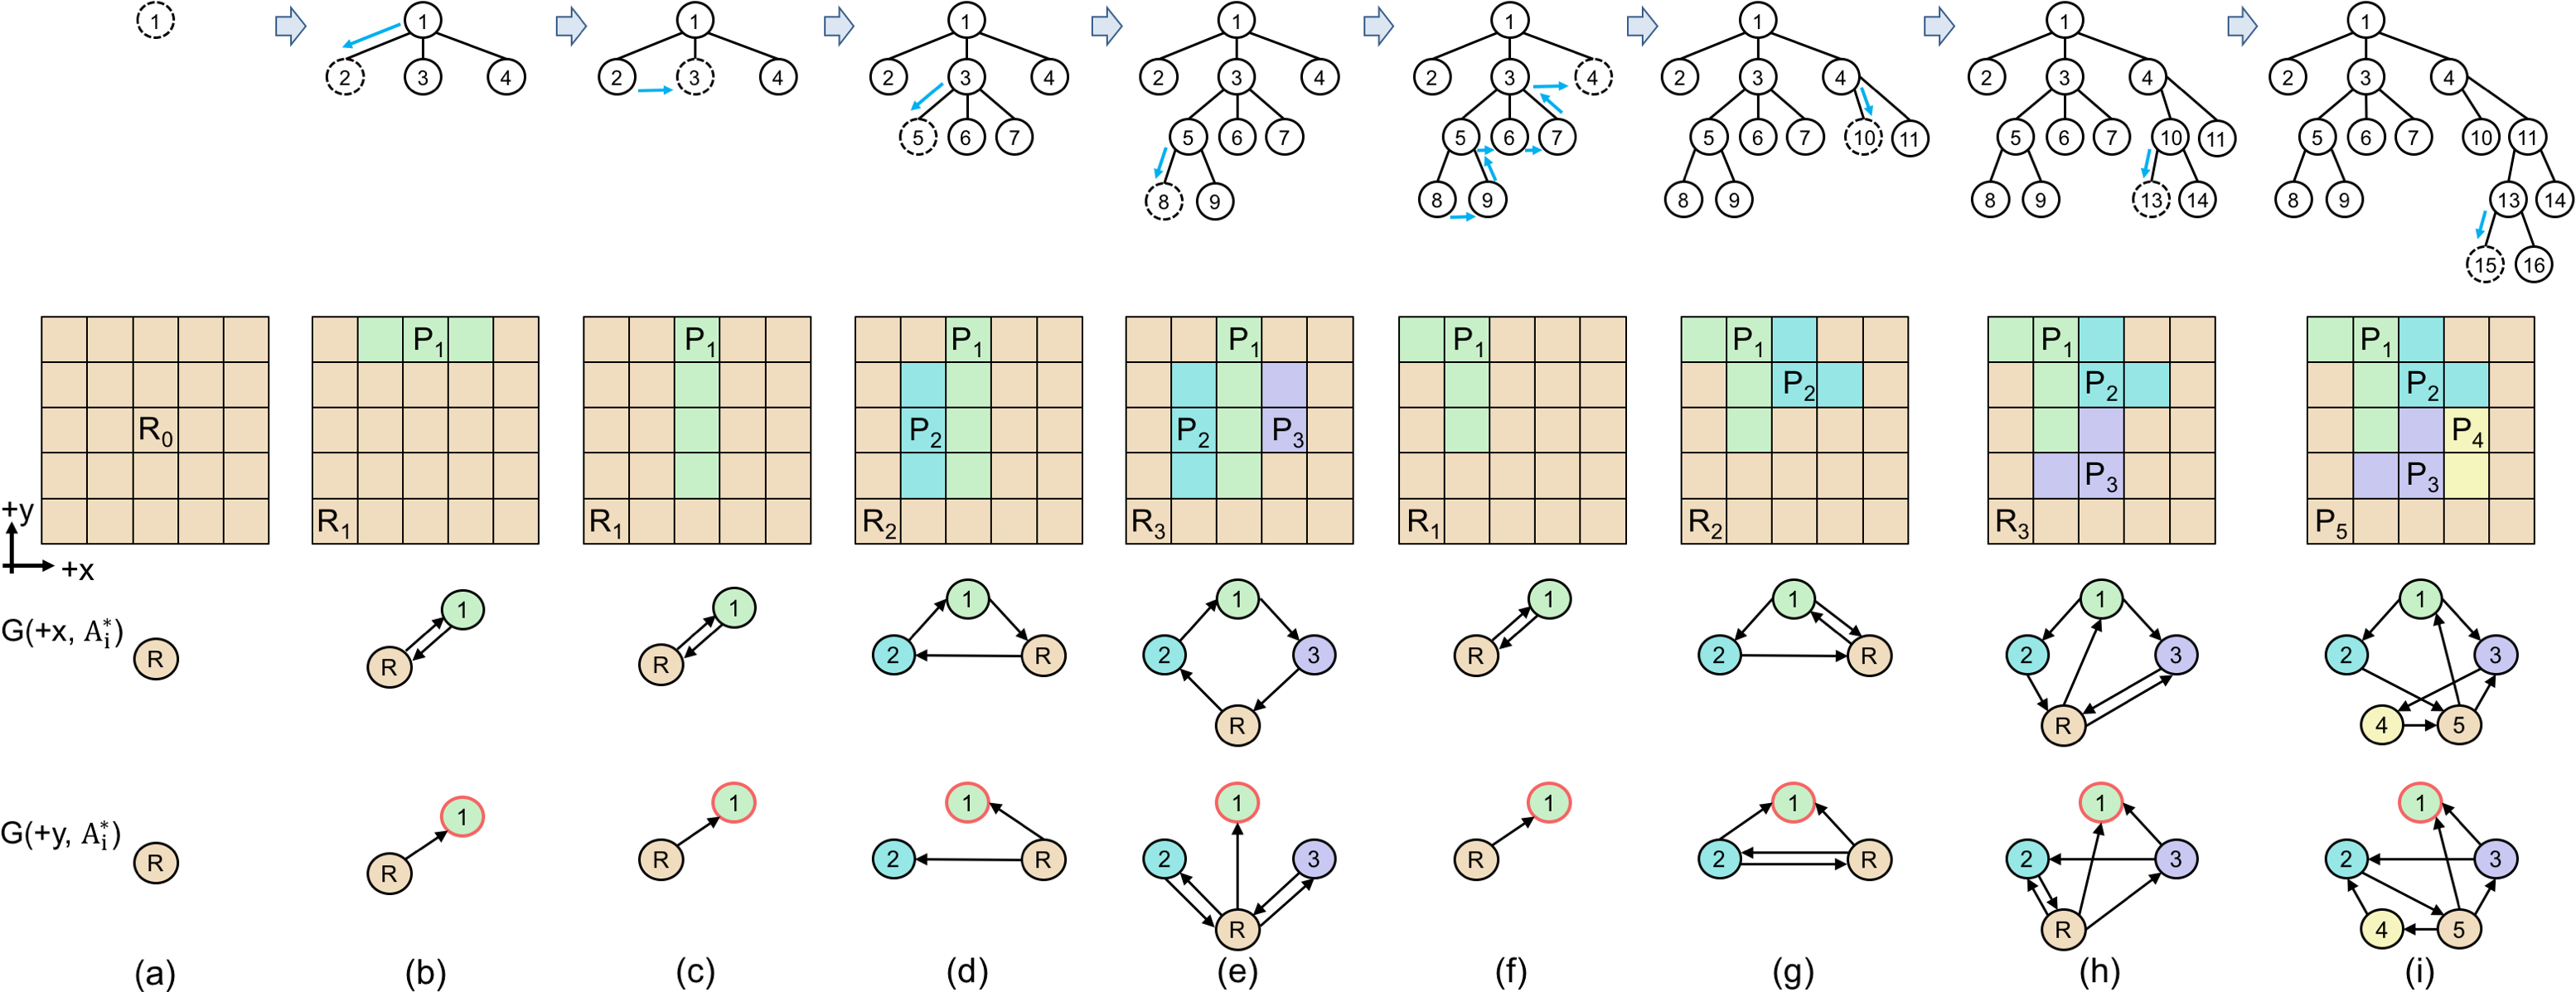
\includegraphics[width=17.80cm]{images/Framework_Overview.png}
	\vspace*{-2.5mm}
	\caption{		
		Overview of our framework on a 2D interlocking design.
		(a) Given a $5 \times 5$ square as input, (b-i) our framework tries to generate a 5-part interlocking 2D assembly, in which each part should have at least two pixels.
		Top row: Construction tree, where each node at depth $i$ represents a candidate of $\mathbf{A}_i$.
		%Each node can have at most $M=3$ children, and the leftmost child in the tree has the highest ranking.
		Here we show the $M=3$ highest ranked options at each level with the top-ranked on the left.
		%\Mark{Maybe better "Here we show the $M=3$  highest ranked options with the top-ranked on the left." We don't want to imply that $M=3$ is some fixed threshold.}		
		The blue arrows indicate the procedure to visit the nodes for generating parts. 
		If the framework cannot find any child for the current node (in dashed circle, denoted as $\mathbf{A}_i^*$), it will backtrack to (c) its siblings or (f) ancestors.
		Middle row: Geometric examples corresponding to the dashed node in the tree.
		Bottom row: Base DBGs of the geometric examples, where the key is indicated by a red circle. For simplicity, we show nodes $P_j$ ($j\leq i$)  as $j$, and $R_i$ as $R$.
		%\Mark{I would add more vertical spacing between the rows.}
	\vspace*{-3.0mm}
	\label{fig:Framework_Overview}}
\end{figure*}


\vspace*{1.0mm}
\noindent
{\bf Non-directional Blocking Graph (NDBG).} \
We represent the set of all translation directions in 2D by the unit circle denoted as $C$.
For every pair of parts in contact in $\mathbf{A}$, we draw the diameter that is parallel with the contact line.
The drawn diameters partition $C$ into an arrangement of regions, for which the corresponding DBG $G(d, A)$ remains constant when $d$ varies over a region.
For any pair of parts in 
%\vspace*{-1mm}
\setlength{\columnsep}{13pt}
\begin{wrapfigure}{r}{0.32\columnwidth}
	\vspace{-6pt}
	\centering
	\hspace{-4pt}
	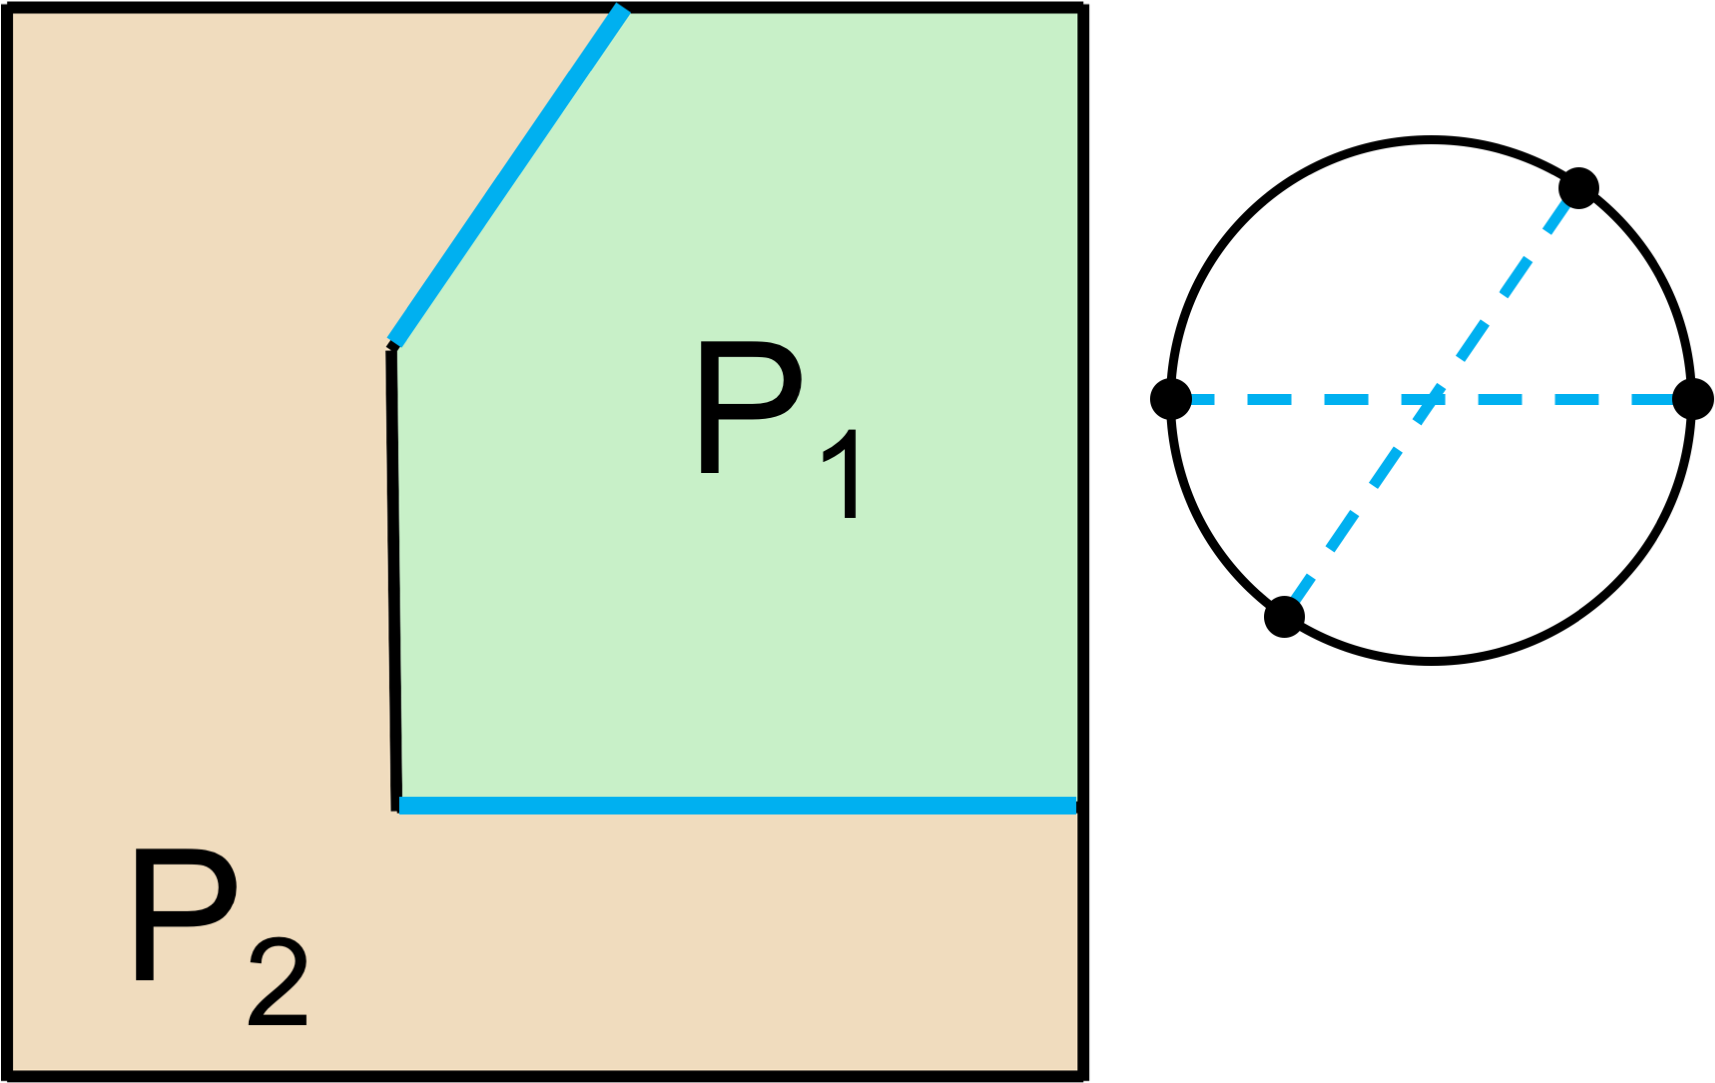
\includegraphics[width=0.32\columnwidth]{images/NDBG_Diameter.png}
	\vspace{-5pt}
\end{wrapfigure}
contact (e.g., $P_1$ and $P_2$ in the inset), if there are more than two contact lines, we only retain the two diameters of $C$ (e.g., two contact lines in blue) which bound the cone of directions in which one part is free to translate relative to the other.
The arrangement of points and intervals on $C$ and the associated DBGs form the {\em non-directional blocking graph} of $\mathbf{A}$; see Figure~\ref{fig:NDBG}(e).
% which represents the blocking relations among parts in $\mathbf{A}$ for all possible translation directions.
The NDBG for a 3D assembly can be built similarly by constructing DBGs for each regular region of a unit sphere that represents all possible translation direction in 3D; please refer to~\cite{Wilson-1994-GeometricReasoning} for more details.



\vspace*{1.0mm}
\noindent
{\bf Base Directional Blocking Graphs.} \
An NDBG represents the parts blocking relations with redundancy in two aspects.
First, the DBG corresponding to an arc in $C$ can be derived by performing union operations on the DBGs associated with the two end points of the arc; see again Figure~\ref{fig:NDBG}(e).
%This is because the blocking relations for $d = d_1$ and $d = d_2$ are the extreme case
%by performing union of the edges in these two graphs since \TODO{give a reason here}.
Second, we can obtain $G(-d, A)$ from $G(d, A)$ easily by reversing the direction of every edge in $G(d, A)$ due to the reciprocity of  blocking relations among the parts.

Therefore, it is sufficient to model the blocking relations in $\mathbf{A}$ by using only a set of {\em base DBGs} denoted as $\{G(d, A)\}$, which we select as the DBGs corresponding to the end points in a half circle of $C$.
For example, two DBGs in Figure~\ref{fig:NDBG}(c\&d) form $\{G(d, A)\}$.
We call the set of directions corresponding to the base DBGs as {\em base directions}, denoted as $\{d\}$.
%The number of base DBGs (as well as base directions) is $O(n^2)$ since every pair of parts provides either two (in contact) or zero (no contact) diameters in $C$.
The number of base DBGs (as well as base directions) is $O(n^2)$ since every pair of parts provides at most two diameters in $C$.  
%\Mark{Does this mean two contact parts cannot be blocked only along a single direction?}
%\Peng{You are right. Two contact parts are possible to provide one diameter. Text has been revised accordingly.}
%\Mark{better to have a figure showing 3D base DBGs}

%Hence, if a part of part group is movable along the direction within the arc, it must be movable also along the direction corresponding to one of the end points.
%Hence, when identifying movable parts or part groups,  we only need to test each direction corresponding to the end points (e.g., $-x, +x, -y, +y$ in Figure~\ref{fig:NDBG}).



%%%%%%%%%%%%%%%%%%%%%%%%%%%%%%%%%%%%%%%%%%%%%%%%
% Test Interlocking 
%%%%%%%%%%%%%%%%%%%%%%%%%%%%%%%%%%%%%%%%%%%%%%%%

\subsection{Testing Interlocking}
In an interlocking assembly, every part and every part group are immobilized for all possible translation directions, except a single key.
To test immobilization of a part group $\mathbf{S}$, we need to compute blocking relations between $\mathbf{S}$ and $\mathbf{A}-\mathbf{S}$:  the part group $\mathbf{S}$ is immobilized if $\mathbf{S}$ is blocked by $\mathbf{A}-\mathbf{S}$ in all translation directions.
Explicitly testing interlocking by checking immobilization of every part and every part group has exponential time complexity. 
However, treating each part group $\mathbf{S}$ independently ignores significant redundancies in the blocking relations across the parts.
%This huge complexity mainly arises from the redundancy of recomputing blocking relations for every parts group $\mathbf{S}$ by considering it as a totally new unit.
% rather than utilizing the computed blocking relations of $\mathbf{S}$'s component parts.
%
We exploit these redundancies and propose a more efficient approach to test global interlocking. 
The key idea is to utilize the blocking relations encoded in the set of base DBGs to implicitly test immobilization of every part and every part group along a finite number of translation directions, i.e., the base directions $\{d\}$.
In detail, an assembly with at least three parts is interlocking, if all base DGBs are either

\begin{enumerate}
\item strongly connected, or 
\item have only two strongly connected components one of which has a single part that is identical across all DGBs.
\end{enumerate}	
%\vspace*{-0.5mm}
Here the strongly connected component with a single part is the key of the assembly.
The direction $d$ associated with each DBG with two strongly connected components is the key part's (reversed) movable direction according to the in-edge (out-edge) of the key in the DBG.
For example, the assembly in Figure~\ref{fig:NDBG}(a) is interlocking and $P_1$ is the key since its two base DBGs in Figure~\ref{fig:NDBG}(c\&d) satisfy the above requirement.
% where $P_1$ is the key part and its movable direction is $\{d_2\}$.

In our implementation, we use Tarjan's algorithm~\cite{Tarjan-1972-SCC} to find the strongly connected components in each DBG. Runtime complexity is linear in the number of edges and nodes in the graph, i.e., $O(n^2)$ since there are at most $n^2$ edges in the graph.
As the set of base DBGs has $O(n^2)$ graphs, the worst-case complexity of our interlocking testing algorithm is $O(n^4)$, which is much lower than $O(2^n)$ of the previous approach~\cite{Song-2012-InterCubes}.
In particular, the complexity to test interlocking of a well-structured assembly, 
where each part connects with at most $L\ll n$ parts, is $O(L^2n^2)$ since the number of base DBGs is $O(Ln)$ and running Tarjan's algorithm on each DBG is also $O(Ln)$.
In practice, our algorithm is extremely fast. For example, our implementation can test for interlocking of the 80-piece \textsc{Bunny} assembly in Figure~\ref{fig:Result_Puzzle_Bunny}(b) in 1 millisecond, including the construction of all blocking graphs. For comparison, the approach of~\cite{Song-2012-InterCubes} takes 24.6 seconds on a 20-piece \textsc{Bunny} of the same voxel count and would run years on the 80-piece model.
See also Section~\ref{sec:results}.

%Our observation is that although the immobilization of a parts group $S$ cannot be derived from those of parts in the group, the blocking relations of the $S$ indeed can be derived.
 
%By using the based DBGs, we can consider an assembly as interlocking if all base DBGs are strongly connected, except a few ones where there is only a common node that does not have out-edges.
%Here, the common node is the key part while the directions associated with the non strongly connected DBGs are the key's movable directions.  



%%%%%%%%%%%%%%%%%%%%%%%%%%%%%%%%%%%%%%%%%%%%%%%%
% Test Disassemblability 
%%%%%%%%%%%%%%%%%%%%%%%%%%%%%%%%%%%%%%%%%%%%%%%%

\vspace*{1.0mm}
\noindent
{\bf Testing Disassemblability.} \
The DBGs were originally developed to test whether a structure can be (dis)assembled.
%The key observation is that a sub-graph (usually a strongly connected component) in a base DBG $G(d,A)$ with zero out-degree (in-degree) is movable along $d$ ($-d$).
%Hence, we can use the Algorithm~\ref{alg:DisasssTest} to find a sequence to disassemble parts in a 2D/3D assembly.
By successively identifying the movable part (or part group) based on the DBGs, we can find a sequence to disassemble all the parts. 
Otherwise, we consider the structure as not (dis)assemblable by translational part motions.

In practice, a part $P$ may not be able to be taken out by a single translation, say along $d$, since some part may block $P$ after it 
moves along $d$ for a certain distance; see the inset figure.
Since this case has 
\setlength{\columnsep}{13pt}
\begin{wrapfigure}{r}{0.30\columnwidth}
	\vspace{-12pt}
	\centering
	\hspace{-8pt}
	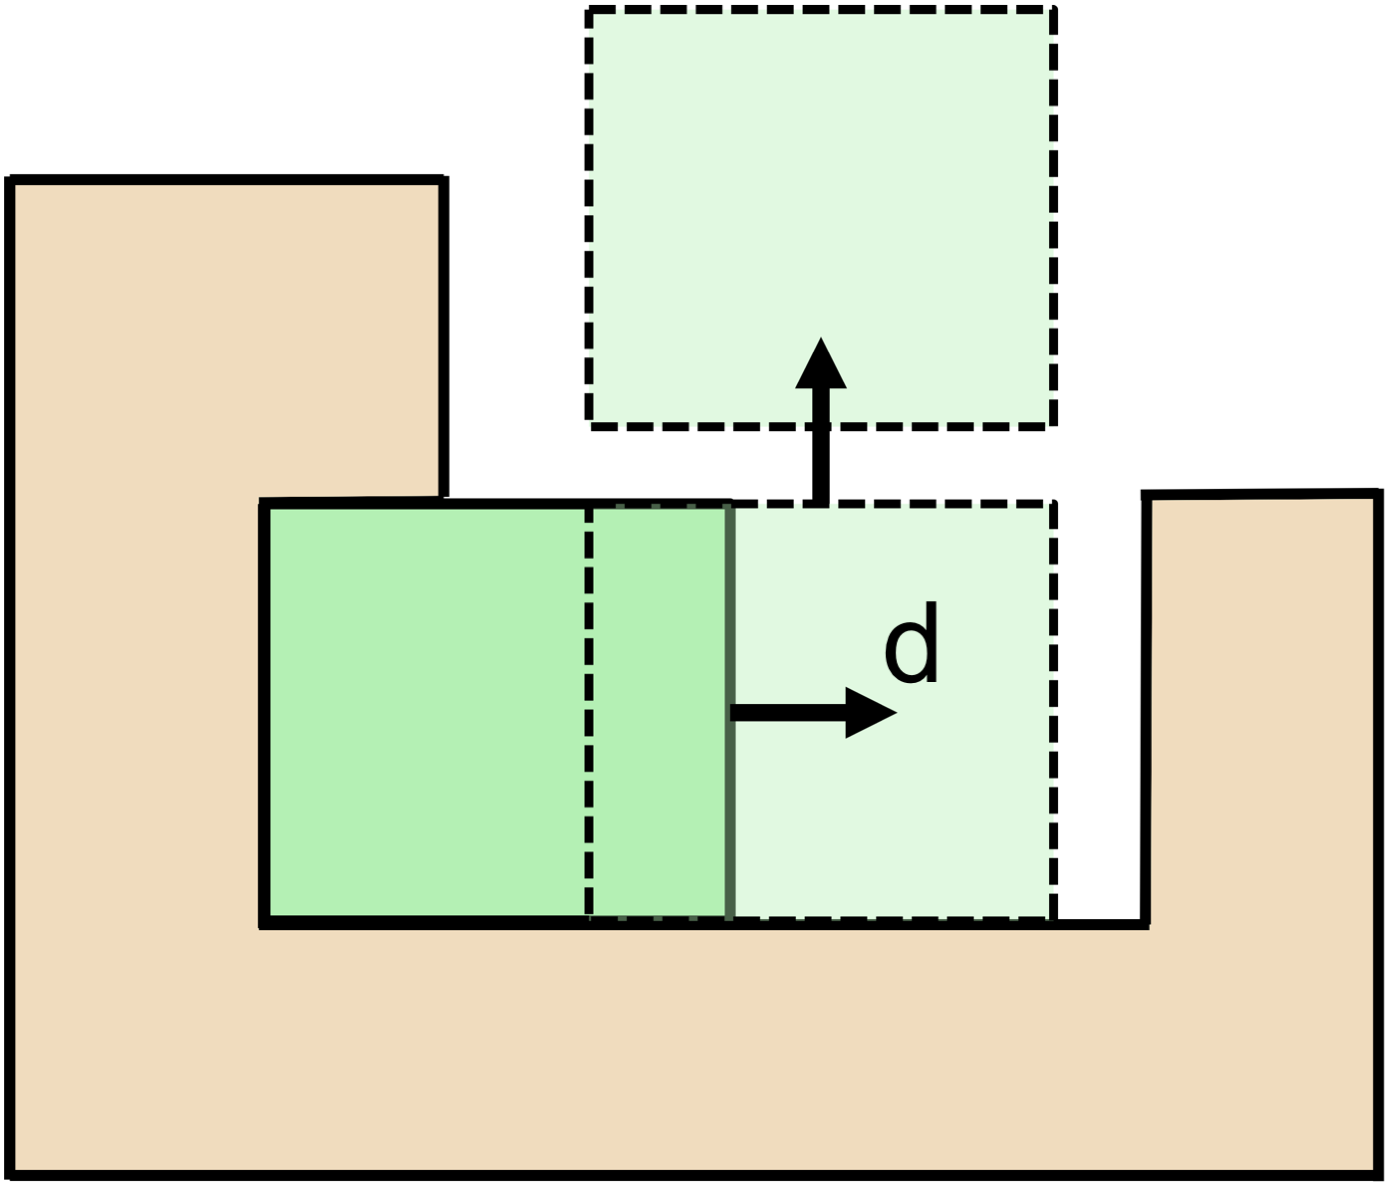
\includegraphics[width=0.28\columnwidth]{images/Multi_step.png}
	\vspace{-11pt}
\end{wrapfigure}
not been modeled in the DBGs, we use a sample-based approach to find a disassembly path of $P$ without parts collision.
%if $P$ cannot be directly taken out along $d$.
Alternatively, more complex disassembly path planning approaches, e.g.~\cite{Ghandi-2015-AssemblyPlanningReview}, could be employed here.










%%%%%%%%%%%%%%%%%%%%%%%%%%%%%%%%%%%%%%%%%%%%%%%%%%%%%%%%%%%%%%%%%%%%%%%%%%%%%%%%%%%%%%%%%%%%%%%%%%%
% Backup
%%%%%%%%%%%%%%%%%%%%%%%%%%%%%%%%%%%%%%%%%%%%%%%%%%%%%%%%%%%%%%%%%%%%%%%%%%%%%%%%%%%%%%%%%%%%%%%%%%%

\if 0
\vspace*{-2mm}
\begin{algorithm}
	\caption{TestDisassemblability($\mathbf{A}$)\ \vspace*{-2mm}}
	\label{alg:DisasssTest}
	\vspace*{1.0mm}
	\KwIn
	{
		\hspace{3.0mm}A 2D/3D assembly $\mathbf{A}$ \\
	}
	\vspace*{0.5mm}
	\KwOut
	{
		\hspace{0.1mm} Disassemblability of $\mathbf{A}$
	}
	\vspace*{2mm}
	Construct a set of base DBGs for $\mathbf{A}$ \;
	\While{ $\mathbf{A}$ is non-empty }
	{
		\vspace*{0.5mm}
		\If{Find a part $P$ whose out-degree (in-degree) is zero in one base DBG $G(d, A)$ }
		{
			Remove $P$ from $\mathbf{A}$ by tranlsating it along $d$ ($-d$) \;
			Update all base DBGs for the new $\mathbf{A}$ \;	
		}
		\ElseIf{Find a parts group $\mathbf{S}$ which is a stongly connected component  in one base DBG $G(d, A)$ and whose out-degree (in-degree) is zero in the DBG}
		{
			\If{TestDisassemblability($\mathbf{S})$ == true }
			{
				Remove parts in $\mathbf{S}$ together from $\mathbf{A}$ along $d$ ($-d$)  \;
				Update all base DBGs for the new $\mathbf{A}$ \;	
				Disassemble parts from $\mathbf{S}$ \;
			}
			\Else
			{
				Return false \;	
			}
		}
		\Else
		{
			Return false \;
		}
	}
	
	Return true \;
\end{algorithm}
\fi









